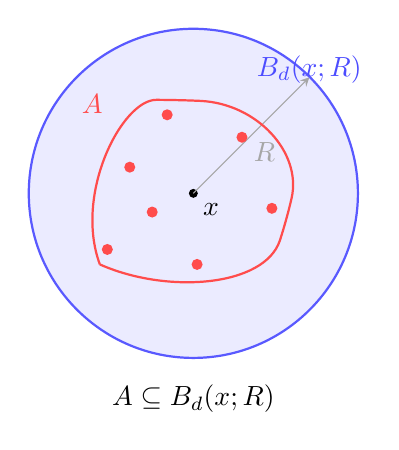
\begin{tikzpicture}[scale=0.95,>=stealth]
  \fill[blue!8] (0,0) circle (2.2);
  \draw[blue!65,thick] (0,0) circle (2.2);
  \node[blue!70] at (1.55,1.65) {\(B_d(x;R)\)};

  \fill[black] (0,0) circle (1.7pt);
  \node[below right] at (0,0) {\(x\)};
  \draw[->,gray!70] (0,0) -- (1.55,1.55);
  \node[gray!70] at (0.95,0.55) {\(R\)};

  \foreach \p in {(-0.85,0.35),(-0.35,1.05),(0.65,0.75),(1.05,-0.2),
                  (0.05,-0.95),(-1.15,-0.75),(-0.55,-0.25)}
  {
    \fill[red!70] \p circle (2.1pt);
  }

  \draw[red!70,thick,rounded corners=8pt]
    (-1.25,-0.95) .. controls (-1.6,0.0) and (-0.95,1.25) .. (-0.2,1.25)
    .. controls (0.85,1.2) and (1.45,0.55) .. (1.25,-0.35)
    .. controls (0.95,-1.25) and (-0.35,-1.35) .. (-1.25,-0.95);
  \node[red!70] at (-1.35,1.2) {\(A\)};

  \node at (0,-2.75) {\(A\subseteq B_d(x;R)\)};
\end{tikzpicture}
